% Presentación de la Entrega 2, OII464. Compilar en esta carpeta con:
%   latexmk -pdf main.tex
% Regenerar figuras: python figuras/generar_figuras.py
\documentclass[aspectratio=169,11pt]{beamer}
\usepackage[T1]{fontenc}
\usepackage{lmodern}
\usepackage[spanish,es-nodecimaldot,es-noshorthands]{babel}
\usepackage{booktabs,array}
\usepackage{tikz}
\usetikzlibrary{arrows.meta,calc,decorations.pathreplacing,patterns,positioning}

\definecolor{azul}{HTML}{1F4E8C}
\definecolor{azulmedio}{HTML}{4472C4}
\definecolor{azulclaro}{HTML}{E4EBF6}
\definecolor{tinta}{HTML}{1F2933}
\definecolor{gris}{HTML}{5B6673}
\definecolor{grisclaro}{HTML}{D9DEE4}
\definecolor{bloqueo}{HTML}{B5473C}

\setbeamertemplate{navigation symbols}{}
\setbeamertemplate{itemize items}[circle]
\setbeamercolor{normal text}{fg=tinta,bg=white}
\setbeamercolor{structure}{fg=azul}
\setbeamercolor{itemize item}{fg=azulmedio}
\setbeamercolor{frametitle}{fg=azul}
\setbeamerfont{frametitle}{size=\large,series=\bfseries}
\setbeamerfont{caption}{size=\scriptsize}
\setlength{\leftmargini}{1.1em}
\setbeamertemplate{headline}{%
  \begin{tikzpicture}[remember picture,overlay]
    \node[anchor=north east,inner sep=0pt]
      at ($(current page.north east)+(-0.3cm,-0.22cm)$)
      {
\includegraphics[width=2.25cm]{figuras/logo_pucv.png}};
  \end{tikzpicture}}
\setbeamertemplate{frametitle}{%
  \vspace*{0.1cm}%
  \begin{minipage}[t][1.12cm][t]{0.75\paperwidth}
    \raggedright\usebeamerfont{frametitle}\usebeamercolor[fg]{frametitle}\insertframetitle
  \end{minipage}\par
  \vspace{-0.08cm}{\color{azulmedio}\rule{\textwidth}{0.6pt}}\par}
\setbeamertemplate{footline}{%
  \leavevmode\hspace{0.45cm}{\color{gris}\tiny OII464 · Tabu Search + D-MAB}%
  \hfill{\color{gris}\tiny\insertframenumber}\hspace{0.45cm}\vspace{0.2cm}}

\newcommand{\cifra}[3]{%
  \begin{minipage}[t]{0.31\textwidth}\centering
    {\scriptsize\color{gris}#1\par}\vspace{0.1cm}
    {\LARGE\bfseries\color{azul}#2\par}\vspace{0.1cm}
    {\scriptsize #3\par}
  \end{minipage}}
\newcolumntype{D}[1]{>{\raggedleft\arraybackslash}p{#1}}
\newcolumntype{C}[1]{>{\centering\arraybackslash}p{#1}}

% Beamer no admite macros con parámetros definidas dentro de un frame.
\newcommand{\fila}[2]{\node[anchor=east,text=gris] at (-0.1,#1+0.4) {#2};}
\newcommand{\tramo}[4]{\fill[#4] (#1,0) rectangle (#2,1);
  \node[align=center] at ({(#1+#2)/2},0.5) {#3};}
\newcommand{\detalle}[5]{\fill[#4] (#1,0) rectangle (#2,1);
  \node[align=center,text=#5] at ({(#1+#2)/2},0.5) {#3};}

\title{Programación de cirugías electivas mediante búsqueda tabú y selección adaptativa de movimientos}
\author{José Basualto, Cristopher Dauros y Carlos Ruz}
\date{2 de noviembre de 2026}

\begin{document}

\begin{frame}[plain]
  \begin{tikzpicture}[remember picture,overlay]
    \node[anchor=north,inner sep=0pt] at (current page.north)
      {
\includegraphics[width=\paperwidth]{figuras/encabezado.png}};
  \end{tikzpicture}
  \vspace*{3.75cm}
  \begin{center}
    {\Large\bfseries\color{azul} Programación de cirugías electivas mediante búsqueda tabú y selección adaptativa de movimientos\par}
    \vspace{0.18cm}
    {\normalsize Entrega 2: configuración experimental\par}
    \vspace{0.18cm}
    {\small José Basualto · Cristopher Dauros · Carlos Ruz\par}
    \vspace{0.05cm}
    {\scriptsize\color{gris} OII464: Desarrollo de Diseños Híbridos para Optimización · Prof. Emanuel Vega · 2 de noviembre de 2026\par}
  \end{center}
\end{frame}

\begin{frame}{Mientras un paciente espera, su sala y su anestesista quedan bloqueados}
  \centering
  \begin{tikzpicture}[x=1cm,y=0.55cm,font=\scriptsize]
    \fila{3}{Sala de anestesia}
    \fila{2}{Anestesista}
    \fila{1}{Sala de cirugía}
    \fila{0}{Cirujano}
    \foreach \y in {3,2}{
      \fill[azulmedio] (0,\y) rectangle (3.4,\y+0.8);
      \node[text=white] at (1.7,\y+0.4) {Anestesia};
    }
    \foreach \y/\etiqueta in {3/Bloqueada,2/Reservado}{
      \fill[bloqueo!12] (3.4,\y) rectangle (5.6,\y+0.8);
      \fill[pattern=north east lines,pattern color=bloqueo] (3.4,\y) rectangle (5.6,\y+0.8);
      \node[fill=white,inner sep=1pt,text=bloqueo] at (4.5,\y+0.4) {\etiqueta};
    }
    \foreach \y in {1,0}{
      \fill[grisclaro] (0,\y) rectangle (5.6,\y+0.8);
      \node[text=gris] at (1.7,\y+0.4) {Paciente anterior};
      \fill[azulmedio] (5.6,\y) rectangle (10.2,\y+0.8);
      \node[text=white] at (7.9,\y+0.4) {Cirugía};
    }
    \draw[gris,dashed] (3.4,-0.15) -- (3.4,4.05);
    \draw[gris,dashed] (5.6,-0.15) -- (5.6,4.05);
    \draw[decorate,decoration={brace,amplitude=4pt},thick,bloqueo]
      (3.4,4.1) -- (5.6,4.1) node[midway,above=3pt] {Espera $W_j$};
    \draw[-{Latex},gris] (0,-0.35) -- (10.5,-0.35) node[midway,below] {Tiempo (esquema conceptual)};
  \end{tikzpicture}

  \vspace{0.08cm}
  \begin{itemize}
    \item La anestesia termina, pero la sala de cirugía sigue ocupada.
    \item La primera sala y el anestesista quedan retenidos hasta el traslado.
    \item Ese bloqueo retrasa a los pacientes siguientes y alarga la jornada.
  \end{itemize}
\end{frame}

\begin{frame}{El calendario debe terminar antes sin exceder la espera máxima}
  \begin{itemize}
    \item Cada paciente pasa por anestesia y luego por cirugía.
    \item Salas y personal son compartidos; el planificador asigna profesionales elegibles.
    \item Restricción estricta: la espera nunca supera \texttt{max\_wait}.
    \item Minimizamos un objetivo combinado, sin penalizar desequilibrio de salas.
  \end{itemize}
  \vspace{0.25cm}
  \[
    f(S)=
    \underbrace{C_{\max}}_{\text{fin de la jornada}}
    +\underbrace{10^{-6}\sum_{o} t_o^{\mathrm{ini}}}_{\text{desempate}}
    +\underbrace{0{,}5\sum_{j} W_j}_{\text{espera total}}
    +\underbrace{1{,}4\max_{j} W_j}_{\text{peor espera}}
  \]
\end{frame}

\begin{frame}{Falta medir si D-MAB aporta a Tabu con espera estricta}
  \begin{itemize}
    \item Yu et al. (2024): Q-learning en programación quirúrgica.
    \item Dolatkhah et al. (2026, preprint): D-MAB dentro de un genético.
    \item Yin et al. (2026): Tabu multioperador entre hospitales.
    \item Nicho: D-MAB en Tabu, dos etapas, espera estricta y reparación.
  \end{itemize}
  \vspace{0.25cm}
  \begin{tikzpicture}
    \node[fill=azulclaro,text width=0.96\textwidth,inner sep=8pt,align=left] {%
      {\small\bfseries\color{azul} Pregunta de investigación}\\[0.1cm]
      ¿En qué condiciones la selección adaptativa de movimientos mediante D-MAB mejora
      la calidad, el tiempo o la robustez de Tabu Search frente a elegir los mismos
      movimientos uniformemente?};
  \end{tikzpicture}
\end{frame}

\begin{frame}{Una cartera fija corre dos caminos y conserva el mejor calendario}
  \centering
  \begin{tikzpicture}[font=\scriptsize,
      caja/.style={draw=azulmedio,fill=azulclaro,rounded corners=2pt,align=center,
                   minimum height=0.95cm,inner sep=4pt},
      aprende/.style={caja,fill=azulmedio,text=white,draw=azul},
      flecha/.style={-{Latex},gris,thick}]
    \node[caja,text width=1.55cm] (datos) {Instancia validada};
    \node[caja,text width=2.15cm,right=0.5cm of datos] (ini) {30 soluciones iniciales\\FIFO, SPT, LPT\\y 27 aleatorias};
    \node[caja,text width=2.9cm,above right=0.05cm and 0.75cm of ini.east,anchor=south west] (uni) {Tabu uniforme\\3.030 evaluaciones};
    \node[aprende,text width=2.9cm,below right=0.05cm and 0.75cm of ini.east,anchor=north west] (dmab) {Tabu + D-MAB\\3.030 evaluaciones};
    \node[caja,text width=2.05cm,right=4.75cm of ini] (min) {Menor $f$ factible\\(desempata por $C_{\max}$)};
    \draw[flecha] (datos) -- (ini);
    \draw[flecha] (ini.east) -- (uni.west);
    \draw[flecha] (ini.east) -- (dmab.west);
    \draw[flecha] (uni.east) -- (min.west);
    \draw[flecha] (dmab.east) -- (min.west);
    \node[below=0.06cm of dmab,text=azul] {ML: fase de evolución};
  \end{tikzpicture}

  \vspace{0.32cm}
  \begin{itemize}
    \item ML actúa en la fase de evolución: elige cada movimiento.
    \item Reparto 50/50 y selección final son deterministas.
    \item No empeora el Tabu de 3.030 de su semilla; gasta el doble.
  \end{itemize}
\end{frame}

\begin{frame}{D-MAB aprende en línea qué movimiento proponer a Tabu}
  \[
    a_t=\arg\max_{a}\left[\bar r_a+C\sqrt{\frac{2\ln t}{n_a}}\right],
    \qquad C=0{,}1
  \]
  \begin{itemize}
    \item Cinco brazos: \texttt{swap}, \texttt{insert}, \texttt{room\_1}, \texttt{room\_2}, \texttt{room\_pair}.
    \item Recompensa: mejora del candidato frente al estado local previo.
    \item Normalizada por 2 \% del objetivo inicial, entre 0 y 1.
    \item Page--Hinkley detecta caídas y reinicia solo estadísticas del bandido.
    \item Aprende dentro de cada corrida, sin entrenamiento previo.
  \end{itemize}
\end{frame}

\begin{frame}{Las etapas usan semillas separadas y el protocolo quedó registrado antes}
  \centering
  \begin{tikzpicture}[x=0.113cm,y=0.9cm,font=\fontsize{7.2}{8.4}\selectfont]
    \tramo{0}{20}{Exploración\\0--19\\calibración 0--5}{azulclaro}
    \tramo{20.4}{40}{Validación v1\\20--39}{azulclaro}
    \tramo{40.4}{60}{Validación v2\\40--59}{azulclaro}
    \tramo{60.4}{80}{Carteras\\60--79}{azulclaro}
    \fill[azulmedio] (80.4,0) rectangle (120,1);
    \node[text=white,align=center] at (100.2,0.5) {Entrega 2\\80--119};
    \draw[gris] (80.4,0) -- (0,-0.45);
    \draw[gris] (120,0) -- (120,-0.45);
    \begin{scope}[x=0.339cm,shift={(0,-1.45)}]
      \detalle{0}{4.9}{Tiempos\\80--84}{azulclaro}{tinta}
      \detalle{5.1}{9.9}{Calibración\\85--89}{azulclaro}{tinta}
      \detalle{10.1}{29.9}{Estudio de congestión\\90--109}{azulmedio}{white}
      \detalle{30.1}{34.9}{Piloto\\110--114}{azulclaro}{tinta}
      \detalle{35.1}{40}{Diagnóstico\\115--119}{azulclaro}{tinta}
    \end{scope}
  \end{tikzpicture}

  \vspace{0.2cm}
  \begin{itemize}
    \item Datos sintéticos: 12 instancias estándar y 48 de congestión.
    \item Protocolo registrado en el commit \texttt{a0da669}, antes de ejecutar.
    \item Cada estudio guarda manifiesto con hashes de código e instancias.
    \item Semillas nuevas en un mismo catálogo no miden generalización.
  \end{itemize}
\end{frame}

\begin{frame}{Cuatro comparaciones separan aprendizaje, cómputo y repetición de la búsqueda}
  \centering\footnotesize
  \begin{tabular}{@{}lll@{}}
    \toprule
    Id & Comparación (evaluaciones) & Explicación alternativa que descarta\\
    \midrule
    C1 & D-MAB $-$ Tabu uniforme (3.030) & La mejora viene de Tabu, no de aprender\\
    C2 & Cartera $-$ Tabu prolongado (6.060) & La cartera mejora solo por más evaluaciones\\
    C3 & Cartera $-$ Dos Tabu (6.060) & La cartera mejora por repetir la búsqueda\\
    C4 & D-MAB $-$ UCB1 sin Page--Hinkley (3.030) & El efecto viene de UCB1, no del reinicio\\
    \bottomrule
  \end{tabular}

  \vspace{0.05cm}
  {\scriptsize\color{gris} Líneas base: FIFO, SPT y LPT, que también integran el inicio de Tabu.\par}
  \vspace{0.12cm}
  \raggedright\normalsize
  \begin{itemize}
    \item Primaria: $f$. Secundarias: $C_{\max}$, espera, factibilidad, tiempo, convergencia.
    \item Wilcoxon sobre medias por instancia, Holm sobre C1--C4, bootstrap jerárquico.
    \item Signo: alternativa $-$ referencia; negativo favorece a la alternativa.
    \item Umbral práctico: 0,25 unidades de $f$.
  \end{itemize}
\end{frame}

\begin{frame}{El catálogo original no ejercía presión sobre la espera}
  \begin{columns}[c,onlytextwidth]
    \begin{column}{0.53\textwidth}
      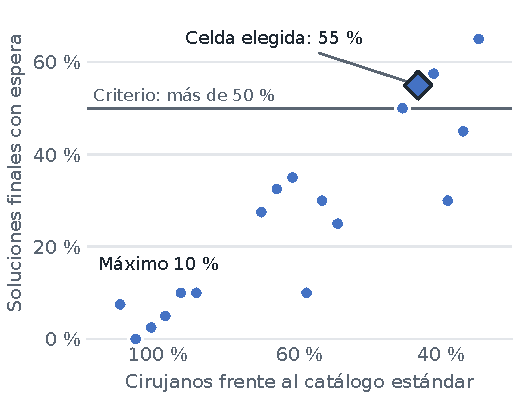
\includegraphics[width=\linewidth]{figuras/calibracion_espera.pdf}
    \end{column}
    \begin{column}{0.44\textwidth}
      \small
      \begin{itemize}
        \item Catálogo estándar: solo 16 de 240 soluciones con espera.
        \item Reducir salas o \texttt{max\_wait} dejó 10 \% o menos.
        \item Reducir cirujanos al 40 \% alcanzó 55 \% en desarrollo.
        \item Con igual sala, la espera depende del cirujano.
        \item Catálogo final: 48 instancias nuevas, 51,8 \% con espera.
      \end{itemize}
    \end{column}
  \end{columns}
\end{frame}

\begin{frame}{240 pares no podían detectar el efecto; la regla previa fijó 960}
  \centering
  \cifra{Planificación, catálogo estándar}{922 pares}{para detectar 0,65 con DE 7,03;\\había 240}\hfill
  \cifra{Regla pre-registrada}{960 pares}{48 instancias por 20 semillas}\hfill
  \cifra{Congestión, DE real 13,21}{Potencia 0,32}{aproximación t para detectar 0,65;\\harían falta 3.246 pares}

  \vspace{0.4cm}
  \raggedright
  \begin{itemize}
    \item Con 12 instancias, la potencia simulada para 0,65 era 0,30.
    \item Con DE 7,03 y aproximación t, bastaban 49 instancias para 0,80.
    \item No ampliamos la muestra: el protocolo prohíbe hacerlo tras ver resultados.
  \end{itemize}
\end{frame}

\begin{frame}{El diseño fija de antemano cómo atribuir una mejora al aprendizaje}
  \begin{columns}[t,onlytextwidth]
    \begin{column}{0.48\textwidth}
      {\bfseries\color{azul} Qué fija este diseño}
      \begin{itemize}
        \item Dos catálogos: 12 estándar y 48 de congestión.
        \item Cinco controles con igual presupuesto de evaluaciones.
        \item Hipótesis, semillas y regla de decisión registradas antes.
      \end{itemize}
    \end{column}
    \begin{column}{0.48\textwidth}
      {\bfseries\color{azul} Qué viene}
      \begin{itemize}
        \item Informar los resultados de C1--C4 en la próxima entrega.
        \item Evaluar igual tiempo, instancias no vistas y mayor escala.
      \end{itemize}
    \end{column}
  \end{columns}
\end{frame}

\appendix

\begin{frame}{Apéndice: la configuración quedó congelada antes de ejecutar}
  \centering\footnotesize
  \begin{tabular}{@{}p{0.17\textwidth}p{0.78\textwidth}@{}}
    \toprule
    Componente & Configuración\\
    \midrule
    Tabu & 30 soluciones iniciales (FIFO, SPT, LPT y 27 aleatorias); lotes de 15 candidatos; memoria de 7 firmas de solución; aspiración por mejora global.\\
    D-MAB & Cinco brazos; $C=0{,}1$; $\delta=0{,}01$; $\lambda=1$.\\
    Cartera & Dos caminos de 3.030 evaluaciones; reparto 50/50 fijo; conserva el menor $f$.\\
    Parada & Agotar el presupuesto de evaluaciones del camino.\\
    Conteo & Cuentan las 30 iniciales y cada candidato distinto del lote, aun infactible. No cuentan duplicados, reparación ni revalidación final.\\
    Entorno & AMD Ryzen 7 8845HS, 8 núcleos, 13,8 GiB; Python 3.13.2, NumPy 2.2.3, SciPy 1.15.2.\\
    \bottomrule
  \end{tabular}
\end{frame}

\end{document}
